\chapter{Evaluation \& Results}

In this chapter we explained how the evaluation of the developed tasks and systems was done.

\section{Sentiment analysis and domain adaptation}

As mentioned previously, the sentiment analysis task was trained using a dataset from Stanford. To perform this task we used the same test and train splits used in \cite{socher2013recursive} which is the same from \cite{DBLP:journals/corr/Kim14f}. During training, both the loss and the prediction accuracy (from a five class prediction, as sen in the previous chapter) of this classification task were recorded (Figure \ref{fig:sa-eval}) but only the loss is used in back-propagation.

The loss function was chosen among the ones available in the Keras framework to be the categorical cross-entropy \cite{golik2013cross} and the optimizer was Adadelta \cite{zeiler2012adadelta}. The batch size was set to 50 to stay as close as possible to the experiment conditions from \cite{DBLP:journals/corr/Kim14f}.

\begin{figure}[h]
    \centering
    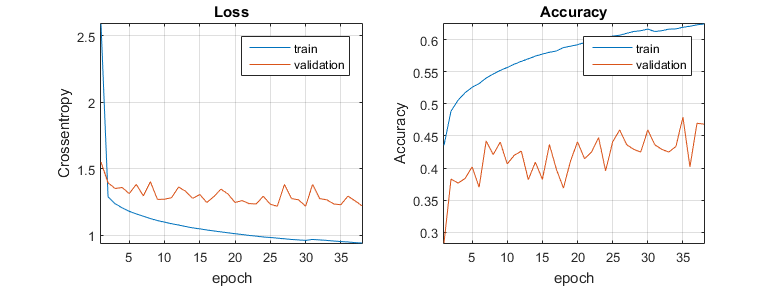
\includegraphics[width=16cm]{figures/sa}
    \caption{Training and validation curves of the sentiment analysis task.}
    \label{fig:sa-eval}
\end{figure}

We obtain 47.9\% accuracy in this task. In \cite{DBLP:journals/corr/Kim14f} they obtain 47.4\% performing the same task with a very similar architecture. Looking at the curves from Figure \ref{fig:sa-eval}, it seems like the model could still be trained for a few more epochs.

The learned function from this model is transferred to the neural network from Table \ref{tab:sent-cnn} using the KL loss as explained in the previous chapter. The optimizer is Adam. The evolution of the KL can be seen in Figure \ref{fig:transfer}.

\begin{figure}[h]
    \centering
    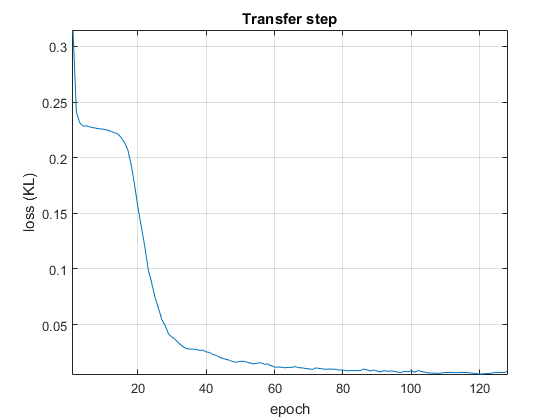
\includegraphics[width=8cm]{figures/transfer}
    \caption{Evolution of the KL loss.}
    \label{fig:transfer}
\end{figure}

From Figure \ref{fig:transfer} we see how the Adam optimizer escapes a local minima. The adaptation from Section \ref{sec:domain} step is performed afterwards, with the weights initialized from this transfer operation. This adaptation is shown in Figure \ref{fig:adap-ev}

\begin{figure}[h]
    \centering
    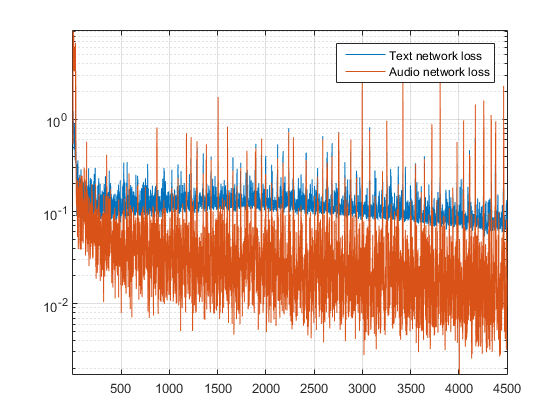
\includegraphics[width=8cm]{figures/adapt}
    \caption{Evolution of the loss function for both the sentiment analysis network (text network in the figure) and the audio based one (audio network).}
    \label{fig:adap-ev}
\end{figure}

Figure \ref{fig:adap-ev} shows that the loss of the adapted sentiment analysis network (Text network in the figure) drops at the beginning but it continues to grow. Despite that, we keep the weights from the 100-th iteration to obtain the adapted embeddings.

\section{Speech synthesis evaluation}

This section contains both the objective and subjective evaluation results and how they were performed. A total of three experiments were evaluated. These experiments are:

\begin{enumerate}
    \item Baseline system (only linguistic features from section \ref{sec:ling-feat})
    \item Embeddings without doing the domain adaptation.
    \item Embeddings but with the domain adaptation.
\end{enumerate}

\subsection{Objective evaluation}

%Training curves of the different stages of this project (accuracy \& loss curves) as well as objective metrics from  the work proposal document.
To perform the objective evaluation the Socrates framework keeps track of the loss evolution during the training. At the end of each batch, it saves the batch loss and at the end of each epoch, the validation data is used to obtain the validation loss of the models.

The metric that are computed by Socrates are the root mean square error (RMSE) for the duration predictions, mel cepstral distortion \cite{mashimo2001evaluation} (MCE) for the MFCC predictions, RMSE for the $F_0$ predictions and accuracy (\%) for the UV flag. 

\begin{table}[h]
    \centering
    \begin{tabular}{|l|c|c|c|c|}
        \hline
                     & Duration &  MFCC & $F_0$ & UV \\
        \hline
        Random weights  & 152.75   & 22.35 & 58.50 & 34.31 \\
        Baseline     & 49.17    & 7.18  & 37.67 & 95.32 \\
        Expressive embeddings     & 51.76    & 7.35  & 41.46 & 94.72 \\
        Adapted embeddings     & 49.37    & 8.24  & 42.04 & 66.28 \\
        \hline
    \end{tabular}
    \caption{Objective metrics.}
\end{table}

Both the duration and acoustic models were trained minimizing the mean square error (MSE) using the Adam \cite{kingma2014adam} optimizer. Figure \ref{fig:loss-dur} contains the training curves of the duration model and Figure \ref{fig:loss-aco} the acoustic model. We see that the baseline system is the one that reaches the lowest loss on both models. The acoustic model shows that the adapted embeddings are the worst in comparison.

\begin{figure}[h]
    \centering
    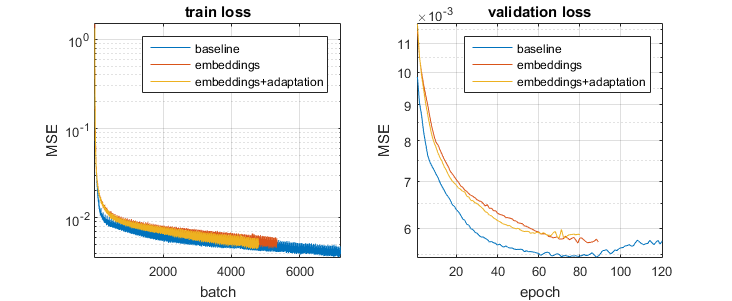
\includegraphics[width=14cm]{figures/duration}
    \caption{Duration model's training curves}
    \label{fig:loss-dur}
\end{figure}

\begin{figure}[h]
    \centering
    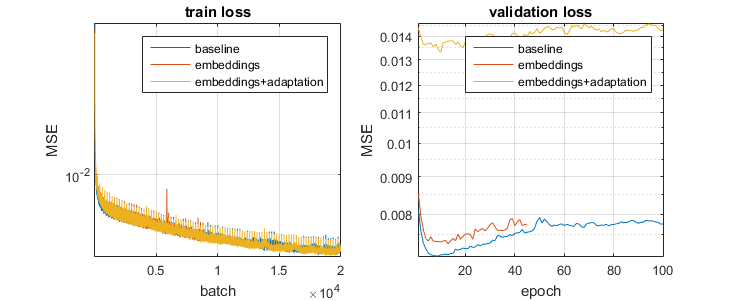
\includegraphics[width=14cm]{figures/aco}
    \caption{Acoustic model's training curves}
    \label{fig:loss-aco}
\end{figure}

\subsection{Subjective evaluation}

%Results from the subjective evaluation. Box plots comparing experiments.
To perform the subjective evaluation, six sentences were chosen from the test split from the Blizzard corpus. To choose the sentences, all the transcripts from the corpus were processed with the sentiment analysis classifier from Section \ref{sec:sa} and a score was computed for each of them:

\begin{equation}
    s = 2 \cdot p_{nn} + \cdot p_{n} - \cdot p_{p} - 2 \cdot p_{pp}
\end{equation}

Where $p_{nn}$ is the probability of the sentence being \textit{very negative}, $p_n$ is the probability of being \textit{negative}, $p_p$ is the probability of the sentence being \textit{positive} and $p_{pp}$ is the probability of being \textit{very positive}. The probability of a sentence being \textit{neutral} is not used in the score.

The scored sentences were sorted in a list and two were picked from the top (as negative sentences), two from the bottom (positive sentences) and two from the middle (neutral sentences).

A web based application (Figure \ref{fig:webapp}) was developed with the selected audio files obtained from the experiments and volunteers were asked to rate how appropriate the voices were in a scale from one to five, one being \textit{very inappropriate} and five being \textit{very appropriate}. The results were saved in an SQL database in the server side of the application.

The test was performed by a total of nine volunteers who gave a rating to all the samples, therefore we end up having a total of fifty-four subjective evaluations for each of the three experiments. Figure \ref{fig:boxplot0} contains a box plot of the collected data:

\begin{figure}[h]
    \centering
    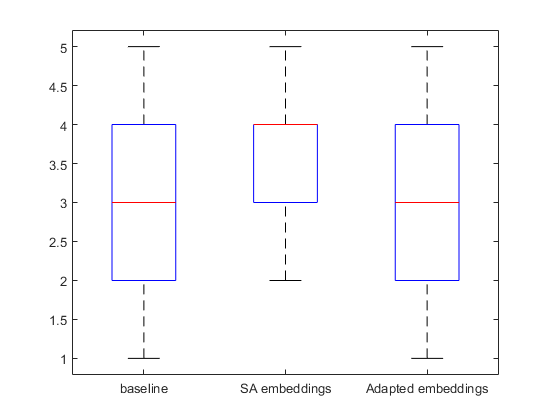
\includegraphics[width=10cm]{figures/box0}
    \caption{Subjective evaluation results.}
    \label{fig:boxplot0}
\end{figure}

Which shows that the expressive experiments have had a more positive reception than the baseline.

\begin{figure}
    \centering
    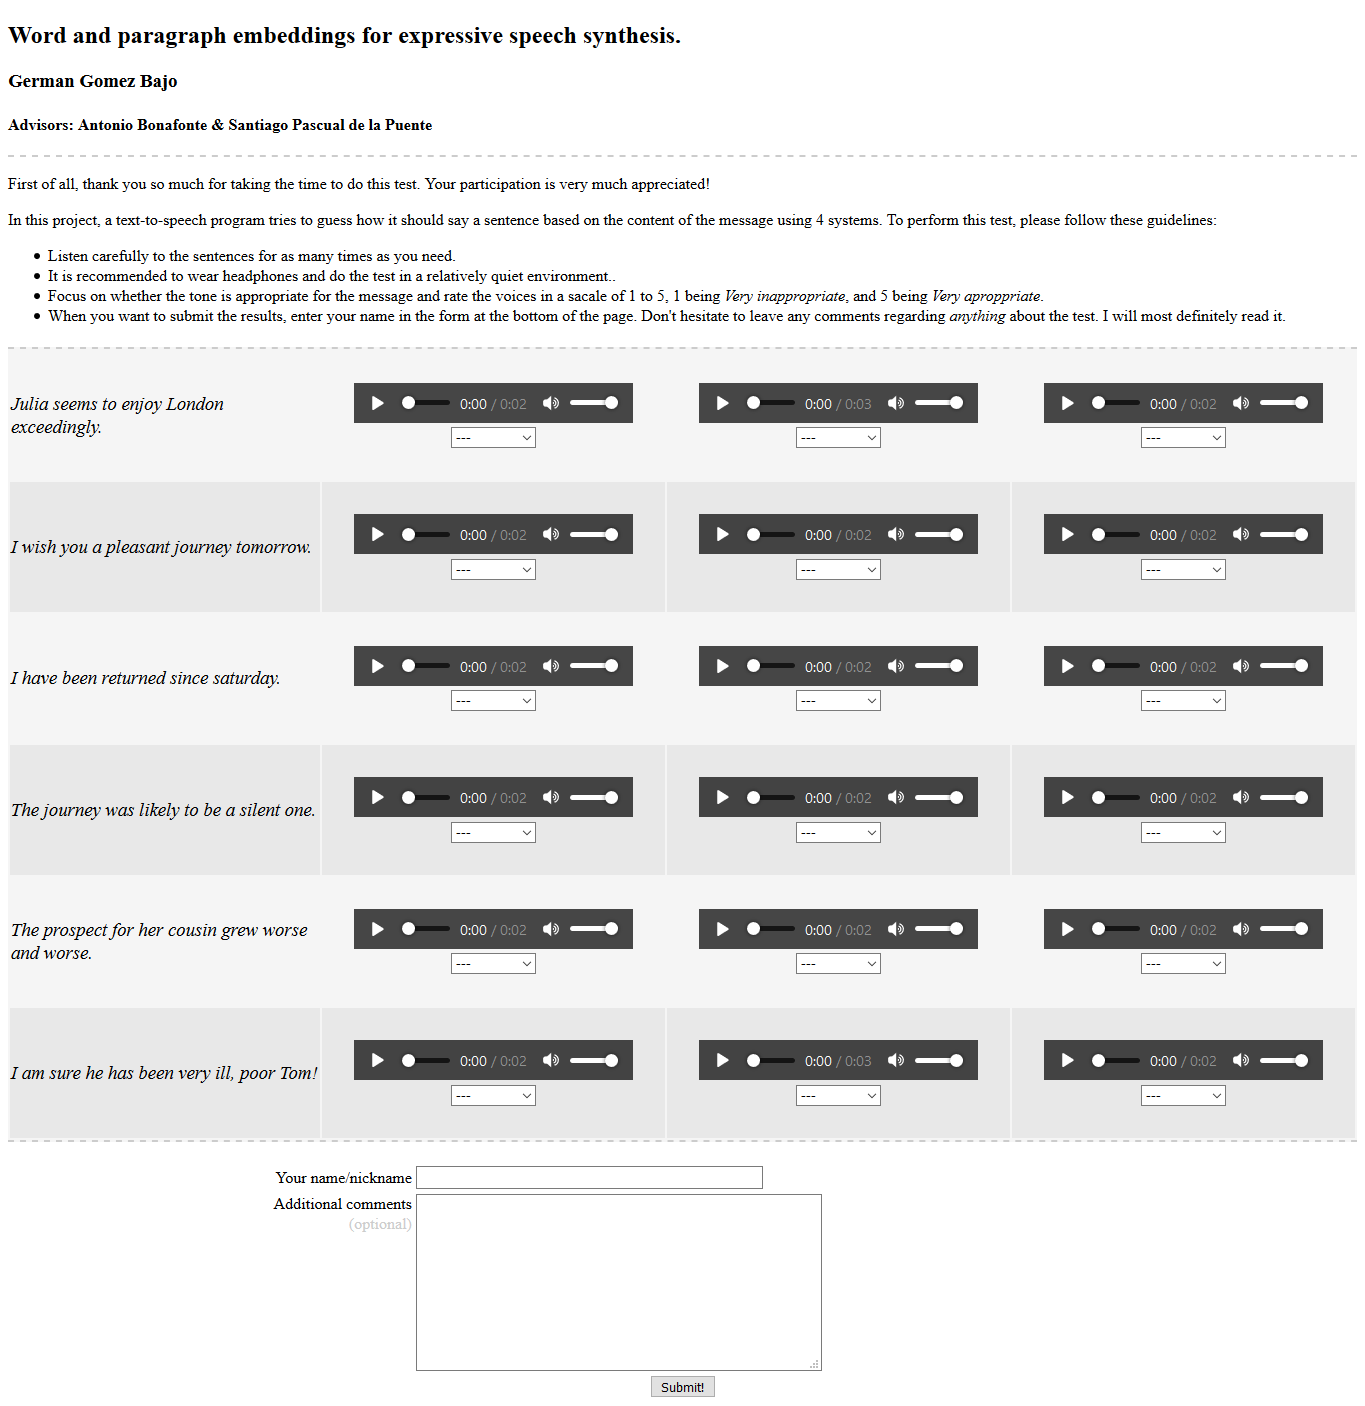
\includegraphics[width=16cm]{figures/webapp}
    \caption{Screenshot of the subjective evaluation's web application.}
    \label{fig:webapp}
\end{figure}
